\vspace*{-2cm}

\part{Statistique}

\setcounter{section}{0}

\section{Vocabulaire}

\begin{tabular}{c|c|c}

Vocabulaire ensembliste & Vocabulaire statistique & Vocabulaire probabiliste \\
\hline
Ensemble & Population & Univers \\
Sous-ensemble & Échantillon & Événement \\
Élément & Individu & Éventualité (cas possible) \\
Propriété & Caractère & {\Large $\times$} \\
\end{tabular} \\

\begin{center}

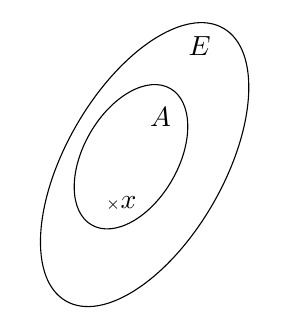
\begin{tikzpicture}
\begin{scope} [rotate=-30]
\draw (0,0)  circle  (1 and 2); 
\draw (0,0) ++(0:-.2) circle (.6 and 1); 
\end{scope} 
\draw (0.7,1.5) node {$E$} ; 
\draw (.2,.6) node {$A$} ; 
\draw (-.3,-.5) node {{\tiny $\times$} $\!\!x$} ; 
\end{tikzpicture}

$ A \subset E $, car A est un sous-ensemble de E.

$ x \in A $ et $ x \in E $ car $x$ est un élément de A, et par conséquent un élément de E. \\

\vspace*{.5cm}

Il existe différents types de caractères : \\

\bigskip 
 
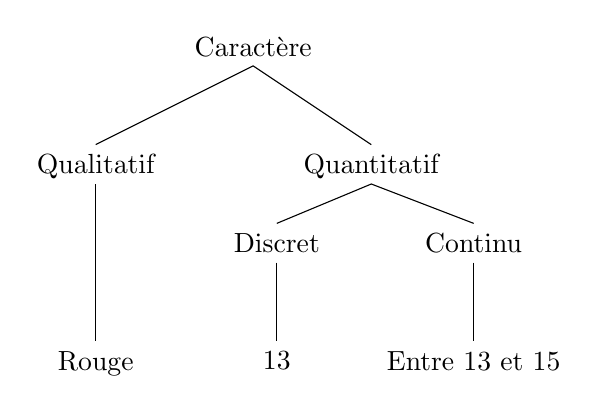
\begin{tikzpicture}
\draw(-2,2) node [below] {Qualitatif} -- (0,3) node [above] {Caractère} 
-- (1.5,2) node [below] {Quantitatif} ; 
\draw (-2,1.5) -- (-2,-.5) node [below] {Rouge} ; 
\draw (0.3,1) node [below]{Discret} -- (1.5,1.5) -- (2.8,1) node [below]{Continu} ; 
\draw (0.3,.5) -- (0.3,-.5) node [below]{13} ; 
\draw (2.8,.5) -- (2.8, -.5) node [below]{Entre 13 et 15} ; 
\end{tikzpicture}
\end{center} 

\vspace*{-.8cm}

\section{La moyenne}

Soit $\left(n_i \;  ;\; x_i\right)$ une série statistique. \\

\begin{tabular}{c|c|c}
Valeur $x_i$ du caractère & Effectifs $n_i$ & $n_ix_i$ \\
\hline
2 & 2 & 4 \\
6 & 7 & 42 \\
10 & 9 & 90 \\
14 & 9 & 126 \\
18 & 1 & 18 \\
\hline
$\Sigma$ & 28 & 280 \\
\end{tabular}

\vspace*{.3cm}

La moyenne de la série statistique est définie par $\overline{x} = \dfrac{\displaystyle{\sum n_ix_i}}{\displaystyle{\sum n_i}}$ \\

Ici, on a $\overline{x} = \dfrac{280}{28} = 10$. 

\vspace*{-5cm}

\newpage

\section{L'écart-type}

\subsection{Introduction}

On observe les résultats en mathématique de 2 élèves, Sylvain et Sylvette, au cours d'un trimestre. On appelle « Élève A » Sylvain, et « Élève B », Sylvette. \\

\begin{itemize}
\item[*] Élève A : $ 11 / 9 / 13 $
\item[*] Élève B : $ 12 / 3 / 18 $
\end{itemize}

\vspace{.3cm}

On constate que $\overline{x_A} = \overline{x_B} = 11 $. \\

\centerline{\footnotesize
\begin{tabular}{c|c|c|c|c|c|c|c|c|c}
& Notes & Moyenne & Écarts & Moyenne & Valeurs & Moyenne & Carrés & Moyenne & Racine \\ 
& & & par & des & absolues & des & des & des & carrée \\
& & & rapport & écarts & des & valeurs & écarts & carrés & de la \\
& & & à la & par & écarts & absolues & par & des & moyenne \\
& & & moyenne & rapport & par & des & rapport & écarts & des \\
& & & & à la & rapport & écarts & à la & par & carrés \\
& & & & moyenne & à la & par & moyenne & rapport & des \\
& & & & & moyenne & rapport & & à la & écarts \\
& & & & & & à la & & moyenne & par \\
& & & & & & moyenne & & & rapport \\
& & & & & & & & & à la \\
& & & & & & & & & moyenne \\
\hline
& & & & & & & & & \\
Élève A & $11$ / $9$ / $13$ & $11$ & $0$ / $-2$ / $+2$ & $0$ & $0$ / $2$ / $2$ & $\dfrac{4}{3} \approx 1,33$ & $0$ / $4$ / $4$ & $\dfrac{8}{3} \approx 2,67$ & $\sqrt{\dfrac{8}{3}} \approx 1,63$ \\
& & & & & & & & & \\
Élève B & $12$ / $3$ / $18$ & $11$ & $+1$ / $-8$ / $+7$ & $0$ & $1$ / $8$ / $7$ & $\dfrac{16}{3} \approx 5,33$ & $1$ / $64$ / $49$ & $38$ & $\sqrt{38} \approx 6,16$ \\
%& & & & RATÉ, il aurait fallu faire une moyenne arithmétique, pas algébrique & & Pas mal, mais pas exploitable & & Ça n'a pas de signification, des points au carré & \\
\hline
& & & & & & & & & \\
& & & & & & & ÉCART-MOYEN & VARIANCE & ÉCART-TYPE \\
\end{tabular}}

\vspace*{.5cm}

\subsection{Définition}

On note l'écart type $\sigma_x$, et on a : $ \sigma_x = \sqrt{\dfrac{\displaystyle{\sum n_i}\left(x_i - \overline{x}\right)^2}{\displaystyle{\sum n_i}}} $.

\subsection{Exemple}

\begin{tabular}{c|c|c|c}
$x_i$ & $n_i$ & $n_ix_i$ & $n_i\left(x_i - \overline{x}\right)^2$ \\
\hline
2 & 2 & 4 & 128 	\\
6 & 7 & 42 & 112 \\
10 & 9 & 90 & 0 \\
14 & 9 & 126 & 144 \\
18 & 1 & 18 & 64 \\
\hline
$\Sigma$ & 28 & 280 & 448 \\
\end{tabular}

\vspace*{.3cm}

$ \overline{x} = \dfrac{\displaystyle{\sum n_ix_i}}{\displaystyle{\sum n_i}} = \dfrac{280}{28} = 10 $ \\

\vspace*{.3cm}

$\sigma_x = \sqrt{\dfrac{448}{28}} = 4 $

\newpage

\vspace*{-2cm}

\subsection{Autre formule}

$ \sigma_x^2 = \dfrac{\displaystyle{\sum n_i \left(x_i - \overline{x}\right)^2}}{\displaystyle{\sum n_i}} $ \\

\vspace*{.5cm}

$ \sigma_x^2 = \dfrac{\displaystyle{\sum n_i\left(x_i^2 - 2\overline{x}x_i + \overline{x}^2\right)}}{\displaystyle{\sum n_i}} $ \\

\vspace*{.5cm}

$ \sigma_x^2 = \dfrac{\displaystyle{\sum n_ix_i^2} - 2\overline{x}\displaystyle{\sum n_ix_i} + \overline{x}^2\displaystyle{\sum n_i}}{\displaystyle{\sum n_i}} $ \\

\vspace*{.5cm}

$ \sigma_x^2 = \dfrac{\displaystyle{\sum n_ix_i^2}}{\displaystyle{\sum n_i}} - 2\overline{x} \dfrac{\displaystyle{\sum n_ix_i}}{\displaystyle{\sum n_i}} + \overline{x}^2 \dfrac{\displaystyle{\sum n_i}}{\displaystyle{\sum n_i}} $ \\

\vspace*{.6cm}

$ \sigma_x^2 = \overline{x^2} - 2\overline{x} \times \overline{x} + \overline{x}^2 \times 1 $ \\

\vspace*{.2cm}

$ \sigma_x^2 = \overline{x^2} - 2\overline{x}^2 + \overline{x}^2 $ \\

\vspace*{.2cm}

$ \sigma_x^2 = \overline{x^2} - \overline{x}^2 $ \\

Et donc $ \sigma_x = \sqrt{\overline{x^2} - \overline{x}^2} $

\section{Variations sur les moyennes et les écarts-type}

\subsection{Changement de variable de type : $X = x + k$}

\begin{itemize}
\item[•] On a $\overline{X} = \overline{x} + k$. \\

\textbf{Preuve :} $\overline{X} = \dfrac{\displaystyle{\sum n_iX_i}}{\displaystyle{\sum n_i}} = \dfrac{\displaystyle{\sum n_i\left(x_i + k\right)}}{\displaystyle{\sum n_i}} = \dfrac{\displaystyle{\sum n_ix_i + kn_i}}{\displaystyle{\sum n_i}} = \dfrac{\displaystyle{\sum n_ix_i}}{\displaystyle{\sum n_i}} + \dfrac{\displaystyle{\sum kn_i}}{\displaystyle{\sum n_i}} = \overline{x} + k$ \\

\vspace*{.3cm}

\item[•] On a $\sigma_X = \sigma_x$. \\

\textbf{Preuve :} $\sigma_X = \sqrt{\dfrac{\displaystyle{\sum n_i\left(X_i - \overline{X}\right)^2}}{\displaystyle{\sum n_i}}} = \sqrt{\dfrac{\displaystyle{\sum n_i\left[\left(x_i + k\right) - \left(\overline{x} + k\right)\right]^2}}{\displaystyle{\sum n_i}}} = \sqrt{\dfrac{\displaystyle{\sum n_i\left(x_i - \overline{x}\right)^2}}{\displaystyle{\sum n_i}}} = \sigma_x$ \\
\end{itemize}

\subsection{Changement de variable de type : $X = kx$}

\begin{itemize}
\item[•] On a $\overline{X} = k\overline{x}$. \\

\textbf{Preuve :} $\overline{X} = \dfrac{\displaystyle{\sum n_iX_i}}{\displaystyle{\sum n_i}} = \dfrac{\displaystyle{\sum n_i\left(kx_i\right)}}{\displaystyle{\sum n_i}} = \dfrac{k\displaystyle{\sum n_ix_i}}{\displaystyle{\sum n_i}} = k\overline{x}$ \\

\vspace*{.3cm}

\item[•] On a $\sigma_X = \abs{k}\sigma_x$. \\

\textbf{Preuve :} $\sigma_X = \sqrt{\dfrac{\displaystyle{\sum n_i\left(X_i - \overline{X}\right)^2}}{\displaystyle{\sum n_i}}} = \sqrt{\dfrac{\displaystyle{\sum n_i\left(kx_i - k\overline{x}\right)^2}}{\displaystyle{\sum n_i}}} = \sqrt{\dfrac{k^2\displaystyle{\sum n_i\left(x_i - \overline{x}\right)^2}}{\displaystyle{\sum n_i}}} = \abs{k}\sigma_x$ \\
\end{itemize}

\vspace*{-5cm}

\newpage

\section{Intérêt de l'écart-type}

Soit $\left(x_i \; ; \; n_i\right)$ une série statistique. \\
Soit $\overline{x}$ la moyenne de cette série. \\
Soit $\sigma_x$ l'écart-type de la série. \\

\begin{tabular}{llll}
\hspace{-.3cm} On étudie la fonction $f:$ & $\R$ & $\longrightarrow$ & $\R$ \\
& $x$ & $\longmapsto$ & $f(x) = \dfrac{1}{\sqrt{2\pi}}e
{\frac{x^2}{2}}$ \\
\end{tabular}

\vspace*{.3cm}

On considère que la répartition est « normale » : \\

\begin{itemize}
\item[*] si les valeurs du caractère comprises entre $\overline{x} - \sigma_x$ et $\overline{x} + \sigma_x$ représentent 68\% de l'effectif total.
\item[*] \textbf{ou} \hbox{si les valeurs du caractère comprises entre $2\overline{x} - 2\sigma_x$ et $2\overline{x} + 2\sigma_x$ représentent 95\% de l'effectif total.}
\item[*] \textbf{ou} \hbox{si les valeurs du caractère comprises entre $3\overline{x} - 3\sigma_x$ et $3\overline{x} + 3\sigma_x$ représentent 99\% de l'effectif total.}
\end{itemize}

\vspace*{.3cm}

%Mettre les dessin.

\begin{tikzpicture}

    \begin{axis}[
      hide y axis, tick align=outside,
      domain=-4:4, samples=50,
%       axis lines*=left, xlabel=Gauss, ylabel=$~$,
        axis lines*=left, xlabel=$~$, ylabel=$~$,
      height=5cm, width=13cm,
      xtick={-4,-3,-1.5,-1,0,1,1.5,3,4}, ytick=\empty,
      xticklabels={%
        $\overline{x}-3\sigma_x$,
        $\overline{x}-2\sigma_x$,
        $\overline{x}-\sigma_x$,
        ,
        $\overline{x}$,
        ,
        $\overline{x}+\sigma_x$,
        $\overline{x}+2\sigma_x$,
        $\overline{x}+3\sigma_x$}      
      ]
   
      \addplot [fill=blue!30, domain=-1.5:1.5] {gauss(0,1)}\closedcycle;
         
            \addplot [thick,red,domain=-4:4] {gauss(0,1)};
   \addplot [red, domain=-4:4] {gauss(0,1)}\closedcycle;
   
         \addplot [thick,green,domain=-3:3] {gauss(0,1)};
      \addplot [fill=VertClair, domain=-3:-1.5] {gauss(0,1)}\closedcycle;   
      \addplot [fill=VertClair, domain=1.5:3] {gauss(0,1)}\closedcycle;

      \addplot [thick,black!50!black,domain=-1.5:1.5] {gauss(0,1)};

    \end{axis}
    
    \draw (5.7,1.5) node {68\%} ;  
    \draw [VertClair](10,3) node {$\bumpeq \; $ 95\%} ;    
    \draw [red](10,2.5) node {$\bumpeq \; $ 99\%} ; 
\end{tikzpicture}

La représentation graphique de la fonction $f$ est appelée « Courbe en cloche de Gauss ». \\

\textbf{Exemple} \\

Si $\overline{x} = 10$ et $ \sigma_x = 4$, alors :

\begin{itemize}
\item[*] $\overline{x} - \sigma_x = 6$ et $\overline{x} + \sigma_x = 14$. On a donc $7 + 9 + 9 = 25$ élèves, soit 89,3\%. 
\item[*] $2\overline{x} - 2\sigma_x = 2$ et $2\overline{x} + 2\sigma_x = 18$. On a donc $28$ élèves, soit 100\%. 
\end{itemize}

\newpage

\section{Exemples}

\subsection{Exemple \no 1 : la taille des bébés}

Dans une maternité, on étudie la taille des bébés en cm pour 200 bébés. \\

\begin{tabular}{rc|c|c|c|c|c}
 & $x_i$ & $n_i$ & $p_i$ & Effectifs cumulés croissants & $n_ix_i$ & $n_ix_i^2$ \\
\cline{2-7}
& 43 & 4 & 2 & 4 & 172 & 7 396 \\
 & 44 & 0 & 0 & 4 & 0 & 0 \\
 & 45 & 0 & 0 & 4 & 0 & 0 \\
 & 46 & 8 & 4 & 12 & 368 & 16 928 \\
 & 47 & 16 & 8 & 28 & 752 & 35 344 \\
 & 48 & 22 & 11 & 50 & 1056 & 50 688 \\
 & 49 & 38 & 19 & 88 & 1862 & 91 238 \\
 & 50 & 42 & 21 & 130 & 2100 & 105 000 \\
 & 51 & 30 & 15 & 160 & 1530 & 78 030 \\
 & 52 & 16 & 8 & 176 & 832 & 43 264 \\
 & 53 & 14 & 7 & 190 & 742 & 39 326 \\
 & 54 & 4 & 2 & 194 & 216 & 11 664 \\
 & 55 & 4 & 2 & 198 & 220 & 12 100 \\
 & 56 & 0 & 0 & 198 & 0 & 0 \\
& 57 & 2 & 1 & 200 & 114 & 6 498 \\
\cline{2-7}
 & $\Sigma$ & 200 & 100 & {\Large $\times$} & 9 964 & 497 476 \\
\end{tabular}

\vspace*{.5cm}

\textbf{Moyenne} \\

$\overline{x} = \dfrac{\displaystyle{\sum n_ix_i}}{\displaystyle{\sum n_i}} = \dfrac{9964}{200} = 49,82$. \\

Donc $\overline{x} = 49,82$cm. \\

\textbf{Écart-type} \\

$\sigma_x = \sqrt{\overline{x^2} - \overline{x}^2} = \sqrt{\dfrac{497476}{200} - \left(\dfrac{9964}{200}\right)^2} \approx 2,31$. \\

Donc $\sigma_x = 2,31$cm. \\

\textbf{Répartition normale} \\

\begin{itemize}
\item[*] $\overline{x} - \sigma_x = 47,51$. \\ $\overline{x} + \sigma_x = 52,13$. \\On a donc $22 + 38 + 42 + 30 + 16 = 148$ bébés, soit 74\%. 
\\
\item[*] $\overline{x} - 2\sigma_x = 45,20$ \\ $\overline{x} + 2\sigma_x = 54,44$. \\ On a donc $200 - 4 - 4 - 2 = 190$ bébés, soit 95\%. 
\end{itemize}

\subsection{Exemple \no 2 : le poids des bébés}

Dans une maternité, on étudie la le poids des bébés en grammes pour 200 bébés. \\

On regroupe les bébés par classes d'amplitude 600. \\

On pose $X_i = \dfrac{1}{100}x_i$. \\

\begin{tabular}{c|c|c|c|c|c|c|c}
Classes & $n_i$ & $p_i$ & Pourcentages cumulés croissants & $x_i$ & $X_i$ & $n_iX_i$ & $n_iX_i^2$ \\
\hline
$[2000,2600[$ & 12 & 6 & 6 & 2300 & 23 & 276 & 6348 \\
$[2600,3200[$ & 64 & 32 & 38 & 2900 & 29 & 1856 & 53824 \\
$[3200,3800[$ & 84 & 42 & 80 & 3500 & 35 & 2940 & 102900 \\
$[3800,4400[$ & 38 & 19 & 99 & 4100 & 41 & 1558 & 63878 \\
$[4400,5000]$ & 2 & 1 & 100 & 4700 & 47 & 94 & 4418 \\
\hline
$\Sigma$ & 200 & 100 & {\Large {$\times$}} & {\Large {$\times$}} & {\Large {$\times$}} & 6724 & 231368 \\
\end{tabular}

\vspace*{.3cm}

\textbf{Moyenne} \\

On a $\overline{X} = \dfrac{\displaystyle{\sum n_iX_i}}{\displaystyle{\sum n_i}} = \dfrac{6724}{200} = 33,62. $ \\

Donc $\overline{x} = 100\overline{X} = 3362$ grammes. \\

\textbf{Écart-type} 

On a aussi $\sigma_X = \sqrt{\overline{x^2} - \overline{x}^2} = \sqrt{\dfrac{231368}{200} - \left(\dfrac{6724}{200}\right)^2} \approx 5,15$. \\

Donc $ \sigma_x = \abs{100}\sigma_X = 515$ grammes.  \\

\textbf{Répartition normale} \\

On a : $\overline{x} - \sigma_x = 2847$ et $\overline{x} + \sigma_x = 3877$ \\

On a ainsi : $ 0 + \dfrac{64 \times 353}{600} + 84 + \dfrac{38 \times 77}{600} + 0 = 126,53$ bébés, soit 63,27\%. \\

La répartition est donc normale.